
\chapter{相关工作与国内外研究现状}
\label{chapter:relate}

\section{文本匹配研究现状}
\label{sec:text_matching}

文本匹配是自然语言处理的一个基础问题。传统的文本匹配算法往往是基于向量空间模型进行的,往往在词汇级别匹配的基础上辅助以各种规则进行处理。这导致整体算法逻辑策略复杂,难以解决语义层面的匹配问题。

近年来,随着计算机计算能力的不断提升,互联网数据的爆炸增长,深度学习相关的算法获得了巨大的发展并开始广泛的应用于图像识别、文本处理等等领域。因此自然而然的,开始有学者试图利用深度学习解决文本匹配问题。

早期文本匹配的深度学习解决方案往往专注于文档的语义表示。通过一个表达函数将一个文档或者句子映射到地位向量空间,并利用一些向量空间的距离函数刻画2个句子的匹配程度。

\begin{figure}[!htbp]\centering
  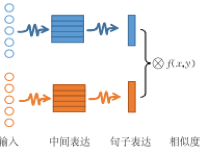
\includegraphics[width=1.0\linewidth]{match_single_doc.png}
  \caption{单文档语义表达匹配框架}{text match based on single document semantics}
  \label{fig:text match based on single document semantics}       % Give a unique label
\end{figure}

深度语义结构模型\cite{Huang2013LearningDS}是最早利用深度学习进行文本匹配的工作,主要是针对查询和文档的匹配任务。它通过搜索引擎里查询和文档的点击日志,利用深度网络得到查询和文档的向量表示,通过余弦相似度计算两个句子的语义相似度,最终得到相似度模型。

深度语义结构模型主要分成3层:输入、表示和匹配层。输入层上对于引文的处理方式为词哈希(word hashing),将每个英文单词切分成 3 个字母为一组的单词。这样可以压缩空间。增强泛化能力;中文以单字的一位有效编码(one-hot)进行输入。在表示层,采用词袋(Bag of words)的方式,输入一个 4 层神经网络,输出 128 维的向量表示,匹配层使用 softmax 进行分类预测。

\begin{figure}[!htbp]\centering
  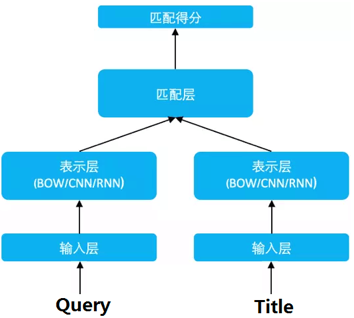
\includegraphics[width=1.0\linewidth]{DSSM.png}
  \caption{深度语义结构模型}{DSSM model}
  \label{fig:DSSM}       % Give a unique label
\end{figure}

图\ref{fig:DSSM} 表示了DSSM的网络结构,图中 $W_i,b_i$ 表示第 $i$ 层全连接的权重。DSSM 使用3个全连接层对文档语义进行建模,最后输出一个 128维的语义向量 $y$:

$$
\begin{aligned}
l_1 &= W_1x\\
l_i &= f(W_il_{i-1} + b_i), i=2,...,N-1\\
y &= f(w_Nl_{N-1} + b_N)
\end{aligned}
$$

我们使用tanh作为隐层和输出层的激活函数:
$$
f(x) = \frac{1-e^{-2x}}{1+e^{-2x}}
$$

最后利用 cosine 距离衡量两个语义向量的相似度:
$$
R(Q, D) = \text{cosine}(y_Q,y_D) = \frac{y_Q^Ty_D}{\|y_Q\|\|y_D\|}
$$
最后通过 softmax 函数将查询与正样本的相似度转化为概率分布:
$$
P(D^+|Q) = \frac{\exp\left(\gamma R(Q, D^+)\right)}{\sum_{D'\in D}\exp\left(\gamma R(Q, D')\right)}
$$
式中的 $\gamma$ 表示平滑因子,$D^+$表示匹配的正样本,其他句子均为负样本(负样本通过在整个文档空间随机采样获得),$D$ 表示整个文档空间。在训练时最小化损失函数

$$
\ell(\Lambda) = -\log \prod_{(Q,D^+)} P(D^+|Q)
$$

这种方法可以减少对切词算法的依赖,提高模型的泛化能力。但是由于使用词袋模型,丧失了语序信息和上下文信息,而且全连接的神经网络参数过多,难以训练。

针对于上面的问题,微软提出了基于单词序列的卷积深度语义模型(CLSM)\cite{Shen2014ALS}。与 DSSM 相比,CLSM 主要对输入和表示层进行了改进。
在输入层上,CLSM加入了一个滑动窗口,利用滑动窗口提取序列信息。

\begin{figure}[!htbp]\centering
  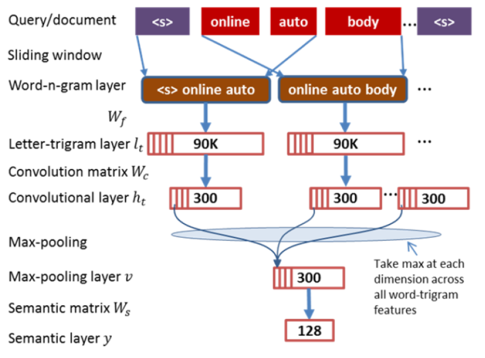
\includegraphics[width=1.0\linewidth]{CLSM.png}
  \caption{CLSM模型结构}{CLSM model}
  \label{fig:CLSM}       % Give a unique label
\end{figure}

在 \ref{fig:CLSM} 的结构中,我们可以看到选择的滑动窗口大小为3。对于一个滑动窗口内的词,类似DSSM,它将每个单词的3-字母组合的词哈希向量相加得到最终的向量表示。原模型中所使用的数据集最终被映射为 9 万维的向量。在表示层上,我们可以看到模型使用了卷积神经网络,利用卷积层的特征进行上下文的特征提取,利用池化层发现全局的上下文特征,最后利用全连接层将结果映射到一个128维的向量空间。这里的激活函数和DSSM相同,也采用了tanh。

在得到了 128 维的向量空间之后,CLSM 也采用了 cosine 距离计算两个语义向量的相似度,在概率分布的转化和损失函数上和 DSSM 都类似,因此不做过多描述。

\begin{figure}[!htbp]\centering
  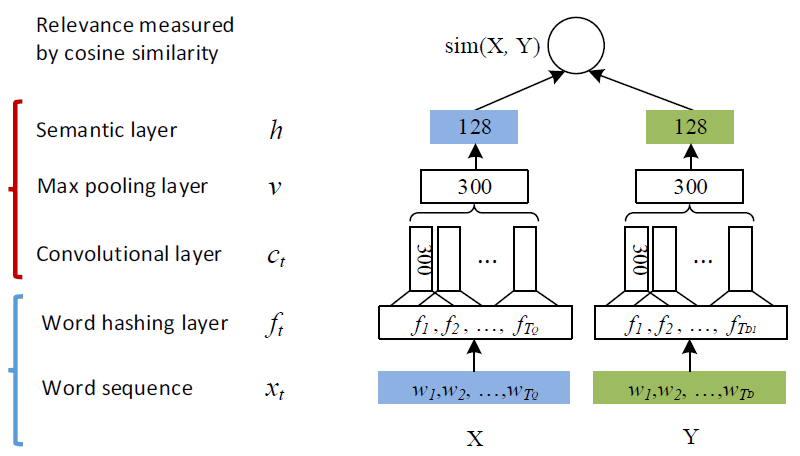
\includegraphics[width=0.8\linewidth]{CLSM_network}
  \caption{CLSM表示层网络结构}{Neural network struct of CLSM}
  \label{fig:CLSM_network}       % Give a unique label
\end{figure}

相对于DSSM,CLSM 通过卷积和池化提取全局的上下文信息,但是对于间隔较远的上下文信息,由于卷积神经网络的限制仍然难以捕捉。

针对于这种问题,有人想到利用 LSTM\cite{Hochreiter1997LongSM}(Long-Short-Term Memory)建模上下文信息,提出了LSTM-DSSM\cite{Palangi2014SemanticMW}。

LSTM是对 RNN(Recurrent Neural Networks) 的改进。RNN是一种用于处理序列信息的神经网络,在处理序列信息是,RNN中每个节点的权值是共享的。

\begin{figure}[!htbp]\centering
  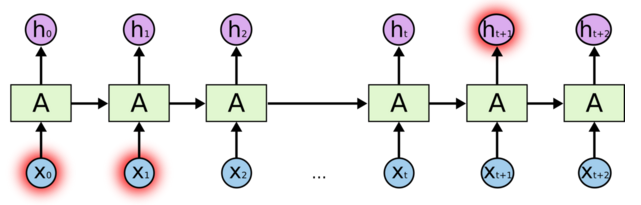
\includegraphics[width=0.8\linewidth]{RNN}
  \caption{RNN 网络结构}{Recurrent Neural Network}
  \label{fig:RNN}       % Give a unique label
\end{figure}

图\ref{fig:RNN} 描述了一个简单的 RNN 网络结构。图中每个节点A的权重都是共享的。但是由于RNN的网络跟序列长度有关,因此当RNN的序列长度过长时,梯度消失的情况会十分明显。这导致 RNN 难以对长序列建模。为了解决这个问题,有人提出了 LSTM:

\begin{figure}[!htbp]\centering
  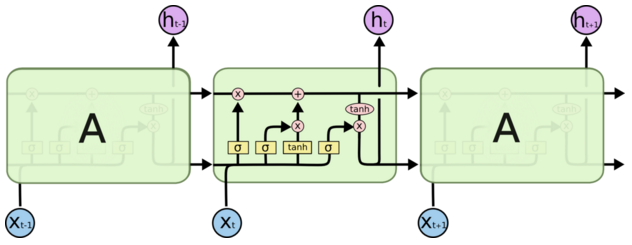
\includegraphics[width=0.8\linewidth]{LSTM}
  \caption{LSTM 网络结构}{Long-Short-Term Memory}
  \label{fig:LSTM}       % Give a unique label
\end{figure}

LSTM 利用遗忘门控制一个节点可以通过的信息量;利用输入们确定要添加到节点的数据;利用输出门确定输出的信息:
$$
\begin{aligned}
f_t&=\sigma(W_f[h_{t-1}, x_t] + b_f) \\
i_t&=\sigma(W_i[h_{t-1}, x_t] + b_i)\\
\tilde{C}_t &= \text{tanh}(W_C[h_{t-1}, x_t] + b_C)\\
o_t&=\sigma(W_o[h_{t-1}, x_t] + b_o)\\
h_t&=o_t\text{tanh}(\tilde{C}_t)
\end{aligned}
$$
通过这种方式,LSTM可以有效避免RNN网络的梯度消失问题。

LSTM-DSSM整体的网络结构为:

\begin{figure}[H]\centering
  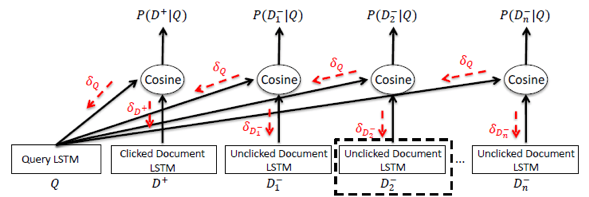
\includegraphics[width=0.8\linewidth]{LSTM-DSSM.png}
  \caption{LSTM-DSSM模型结构}{LSTM-DSSM model}
  \label{fig:LSTM-DSSM}       % Give a unique label
\end{figure}

相对于CLSM,LSTM-DSSM主要是将 CNN 换成了 LSTM。

DSSM本身是端到端的模型,虽然它省下了算法工程师特征工程部分的操作,但是其效果不可控;而且 DSSM 都是弱监督模型,需要大量的训练样本进行训练。在 DSSM论文中,作者提到实际训练所使用的样本量超过一亿,而且论文中所使用的样本都是曝光置信度较高的样本。这些限制因素极大的限制了 DSSM 的使用场景,往往只有少量大公司才可以使用。

这种情况下开始有学者关注于直接利用深度学习建模匹配的模型,提取句子之间的交互特征。这种方式更加直观,也更符合人类判断两个句子是否相似的过程。

MatchPyramid\cite{Pang2016TextMA}利用匹配矩阵建模两个句子的交互过程。匹配矩阵中每个值都是2个句子中词两两计算得到的相似度。相似度可以使用词向量的余弦相似度或点积等进行刻画,而2个词在各自句子中的位置自然组成了一个二维坐标,因此构造出了匹配矩阵。之后将匹配的问题建模为在这个矩阵上进行图像识别的过程,利用卷积和池化操作捕捉局部和全局的交互信息。

\begin{figure}[!htbp]\centering
  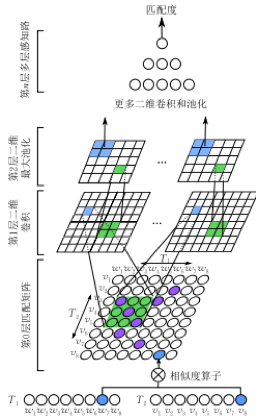
\includegraphics[width=0.4\linewidth]{MatchPramid.png}
  \caption{MatchPramid 模型}{MatchPramid model}
  \label{fig:MatchPramid}       % Give a unique label
\end{figure}

但是和CDSSM类似,利用 CNN 建模文本匹配的过程很可能失去文本的序列信息。因此有人提出了 MatchSRNN\cite{Wan2016MatchSRNNMT},利用 RNN 对匹配矩阵进行建模。但是 RNN 本身只能处理一维序列信息,因此 MatchSRNN 使用了Spatial RNN\cite{Graves2007MultidimensionalRN} 进行建模。Spatial RNN 的每个节点接受4个输入:
$$
\vec{h}_{ij} = f(\vec{h}_{i-1,j},\vec{h}_{i,j-1},\vec{h}_{i-1,j-1},\vec{s}_{ij})
$$
式中 $\vec{h}_{ij}$ 表示在匹配矩阵 $(i, j)$ 位置上的隐状态,$\vec{s}_{ij}$表示在匹配矩阵 $(i, j)$ 位置上的输入。MatchSRNN 使用了RNN的变种 GRU\cite{Cho2014LearningPR}(Gated Recurrent Unit)。 GRU 是对 LSTM 的简化,LSTM 中有三个门:遗忘门、输入门和输出门,GRU中只有两个门:更新门和重置门。更新门和重置门都控制历史状态对当前状态的影响,更新门控制了历史状态进入当前单元的程度,重置门控制了当前状态忽略历史状态。

\begin{figure}[!htbp]\centering
  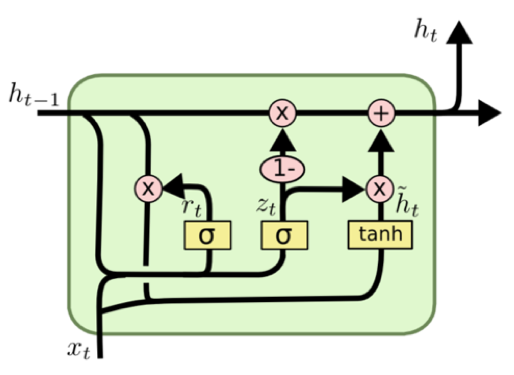
\includegraphics[width=0.8\linewidth]{GRU}
  \caption{GRU 模型}{Gated Recurrent Unitl}
  \label{fig:GRU}       % Give a unique label
\end{figure}

GRU 的计算方式为:
$$
\begin{aligned}
r_t &= \sigma(W_r[h_{t-1},x_t])\\
z_t &= \sigma(W_z[h_{t-1},x_t])\\
\tilde{h}_t &= \text{tanh}(W_{\tilde{h}}[r_t \times h_{t-1},x_t]) \\
h_t &= (1-z_t)\times h_{t-1} + z_t\times\tilde{h}_t
\end{aligned}
$$

Spatial GRU的计算方式为:
$$
\begin{aligned}
&\vec{q}^T = [\vec{h}^T_{i-1,j}, \vec{h}^T_{i-1,j-1}, \vec{h}^T_{i,j-1}, \vec{s}_{ij}^T]^T \\
&\vec{r}_l = \sigma(W^{(r_l)}\vec{q} + \vec{b}^{(r_l)})\\
&\vec{r}_t = \sigma(W^{(r_t)}\vec{q} + \vec{b}^{(r_t)})\\
&\vec{r}_d = \sigma(W^{(r_d)}\vec{q} + \vec{b}^{(r_d)})\\
&\vec{r}^T = [\vec{r}_l^T, \vec{r}_t^T, \vec{r}_d^T]^T\\
&\vec{z}'_i = W^{(z_i)}\vec{q} + \vec{b}^{(z_i)} \\
&\vec{z}'_l = W^{(z_l)}\vec{q} + \vec{b}^{(z_l)} \\
&\vec{z}'_t = W^{(z_t)}\vec{q} + \vec{b}^{(z_t)} \\
&\vec{z}'_d = W^{(z_d)}\vec{q} + \vec{b}^{(z_d)} \\
&[\vec{z}_i,\vec{z}_l,\vec{z}_t,\vec{z}_d] = \text{SoftmaxByRow}([\vec{z}'_i,\vec{z}'_l,\vec{z}'_t,\vec{z}'_d])\\
&\vec{h}'_{ij} = \phi(W\vec{s}_{ij} + U(\vec{r}\odot[\vec{h}^T_{i-1,j}, \vec{h}^T_{i-1,j-1}, \vec{h}^T_{i,j-1}]^T) + \vec{b})\\
&\vec{h}_{ij} = \vec{z}_l\odot\vec{h}_{i,j-1} + \vec{z}_t\odot\vec{h}_{i-1,j} + \vec{z}_d\odot\vec{h}_{i-1,j-1} + \vec{z}_i\odot\vec{h}'_{i,j}
\end{aligned}
$$
式中的 SoftmaxByRow 对每一个维度进行线性变换:

$$
[\vec{z}_p]_j = \frac{e^{[\vec{z'}_p]_j}}{e^{[\vec{z'}_i]_j}+e^{[\vec{z'}_l]_j}+e^{[\vec{z'}_t]_j}+e^{[\vec{z'}_d]_j}}, p=i,l,t,d
$$

MatchSRNN利用 Spatial GRU 对计算整个匹配矩阵,对Spatial GRU 进行全连接层进行非线性变换得到最后的结果。

\begin{figure}[!htbp]\centering
  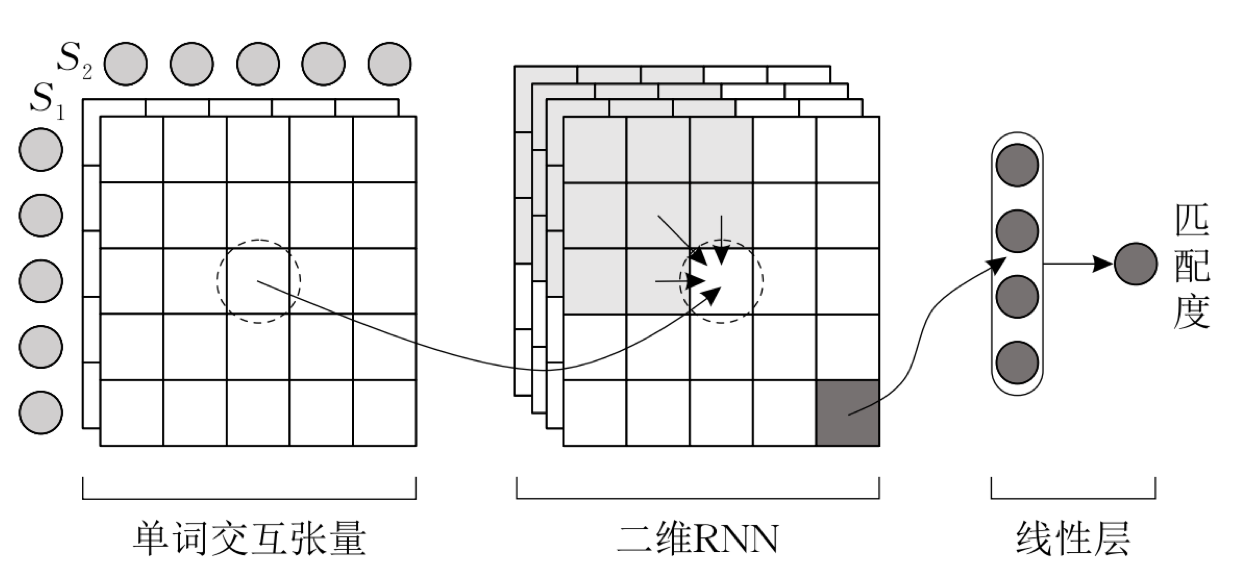
\includegraphics[width=0.8\linewidth]{MatchSRNN}
  \caption{MatchSRNN 模型}{MatchSRNN model}
  \label{fig:MatchSRNN}       % Give a unique label
\end{figure}

\section{强化学习研究现状}
\label{sec:rl_intro}
强化学习\cite{Sutton1998ReinforcementL}是机器学习中的一个重要研究领域,它以试错的机制与环境(Environment)进行交互,通过最大化累积奖赏来学习最优策略。强化学习研究的问题往往有三个特征:闭环性,学习系统产生的行为(action)会影响后续输出;无监督,学习对象只能通过学习得到行为的信息;行动产生的结果,包括奖励(reward),会影响较长时间。

一个强化学习过程可以被定义为一个五元组<$S, A, P, R, \pi$>,其中:
\begin{itemize}
  \item[•] 状态(Status,S)是环境的状态;
  \item[•] 动作(Action, A)是主体在特定环境下使用的策略
  \item[•] 转移概率(Transition function,P)是环境受主体动作影响后状态的迁移概率;
  \item[•] 奖励(Reward,R)是环境根据主体行为返回给主体的信号,主体根据奖励调整自己的策略;
  \item[•] 策略(Policy,$\pi$)定义了特定环境下主体的行为方式,表示状态到动作的映射关系。策略分为确定性和随机性两种。
\end{itemize}

\begin{figure}[!htbp]\centering
  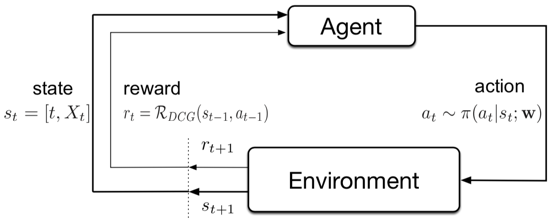
\includegraphics[width=1.0\linewidth]{interaction.png}
  \caption{主体与环境的交互}{interaction between agent and enviroment}
  \label{fig:interaction}       % Give a unique label
\end{figure}

主体和环境的交互可以用图\ref{fig:interaction}表示。主体在当前状态$s_t$下根据策略π选择动作$a_t$,环境接收到该动作并转移到下一状态$s_{t+1}$,主体接收环境反馈回来的奖励选择下一步动作。强化学习不需要监督信号,主要算法包括Q学习(Q-learning),策略梯度(policy gradient)等等。

深度强化学习的主要思路是将神经网络用于抽取复杂高维数据中的信息,并将其映射到一个低维向量空间便于强化学习处理。
由于卷积神经网络在计算机视觉领域的统治地位,DeepMind团队在2013年尝试将卷积神经网络和强化学习结合,提出来深度Q网络(DeepQ Network,DQN)\cite{Mnih2013PlayingAW},并成功的将该方法用在了Atari视频游戏。这是深度强化学习首次在高维度的状态空间下起作用。

2015年,DeepMind团队进一步完善了DQN算法\cite{Mnih2015HumanlevelCT}。
DQN将深度卷积神经网络和Q学习结合到一起,并集成了经验回放技术(memory reply)和目标Q网络。
经验回放通过随机采样系统在探索环境时得到的状态数据对神经网络参数进行更新,打破了Q-学习算法采样数据之间的相关性。DQN在没有任何人类先验知识的情况下在Atari视频游戏表现出了等同人类玩家的水平纪念,是深度强化学习领域的重要工作。

2016年初,DeepMind团队发表了围棋AI:AlphaGo\cite{Silver2016MasteringTG}。AlphaGo 利用强化学习指导蒙特卡罗树搜索的过程,将深度强化学习的研究推向了新的高度。它通过策略网络学习不同位置的落子概率,利用价值网络学习棋局的胜率评估,通过策略和价值网络的结合减小了蒙特卡罗树搜索的搜索次数,提高了搜索效率。在在线对弈时,利用蒙特卡罗树搜索以及策略和价值网确定当前的落子位置。

\begin{figure}[!htbp]\centering
  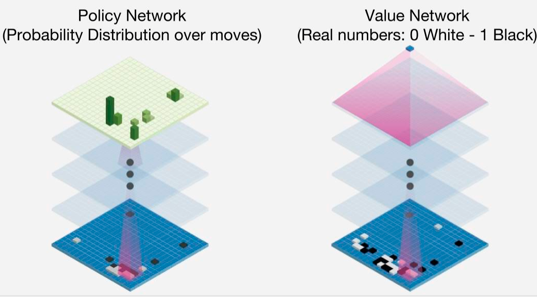
\includegraphics[width=0.8\linewidth]{AlphaGo.png}
  \caption{AlphaGo的策略网络和价值网络} {AlphaGo policy and value network}
  \label{fig:AlphaGo}       % Give a unique label
\end{figure}

2017年初,AlphaGo Zero\cite{Silver2017MasteringTG}对AlphaGo进行了改进和升级。AlphaGo Zero 抛弃了 AlphaGo 复杂的特征输入,只需要将棋局图片作为数据即可;将策略网络和价值网络整合在一起,直接利用深度强化学习方法进行端到端的自我对弈学习。
相比于 AlphaGo,AlphaGo Zero 去除了棋手的落子网络,因此不需要任何先验知识;策略网络和价值网络的整合使得神经网络的复杂度降低,泛化性进一步增强,降低了硬件的资源需求,减少了训练时间。

AlphaGo Zero的成功证明了在没有任何先验经验的情况下,深度强化学习在围棋领域仍然能取得巨大的成功;而在围棋下法上,AlphaGo Zero创造了更多的下棋方式,大大开拓了人类对围棋的认知。
虽然基于蒙特卡罗树搜索的深度强化学习方案已经取得了成功,但是由于搜索算法带来的时间和空间开销,使得其很难满足实时性的需求。目前强化学习很难在星际争霸这种实时游戏上战胜人类。

\begin{figure}[!htbp]\centering
  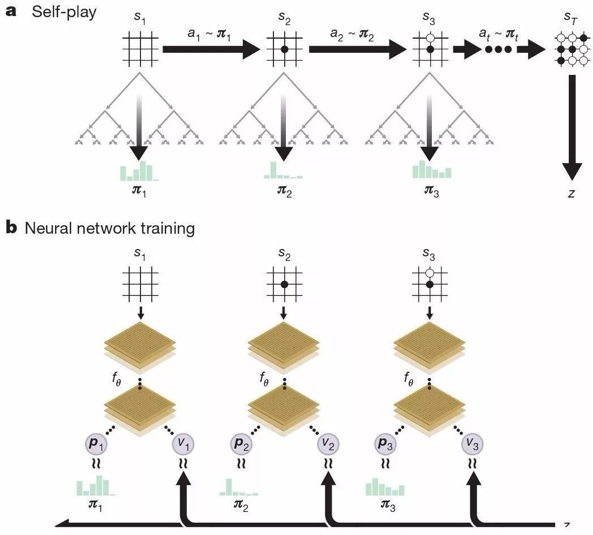
\includegraphics[width=0.8\linewidth]{AlphaGo_Zero.png}
  \caption{AlphaGo Zero 自我对弈训练过程} {training process of AlphaGo Zero}
  \label{fig:AlphaGo_Zero}       % Give a unique label
\end{figure}

\section{本章小结}

本章主要介绍了文本匹配和强化学习的相关工作与研究现状。

本章的第一小节主要介绍了基于深度学习的文本匹配算法。目前基于深度学习的文本匹配算法大都集中于利用神经网络理解输入句子的语义信息。最早利用深度学习解决文本匹配问题是DSSM。DSSM 利用词哈希以及词袋的方式得到句子的向量表示,并利用一个三层的全连接网络将句子的向量表示映射为一个低维向量表示。最后利用余弦相似度计算两个语义向量的距离,并利用 softmax 对得到的结果进行非线性变换,得到最后的概率分布。DSSM 通过词哈希降低了对且此算法的依赖,但是由于词袋模式的使用使其难以捕捉句子的上下文信息,而且全连接网络参数量极大,很难训练。为了解决 DSSM 模型问题,有人提出了CDSSM。相比于DSSM,CDSSM在词哈希的基础上引入了滑动窗口,通过滑动窗口解决了DSSM中上下文信息建模苦难的问题。同时 CDSSM 在表达网络中引入了卷积和池化操作,通过卷积建模上下文特征,利用池化发现全局特征,最后利用一个全连接层将结果映射到一个低维向量空间。但是由于卷积神经网络不是为序列化设置,因此对于长句子的上下文信息,CDSSN仍然难以捕捉。针对这个问题,有人提出将 LSTM 用于表达网络。DSSM及其后续的改进工作虽然有效的提高了文本匹配的效果,但是 DSSM 端到端的学习方式以及弱监督特征决定了它的利用场景十分有限。这种情况下有人提出了直接建模匹配模型的方法。MatchPyramid 利用两个句子之间词的相似度构造了一个匹配矩阵,将文本匹配过程视为对这个匹配矩阵的分类过程。 MatchPyramid 使用 CNN 建模了分类过程。和 MatchPyramid 类似, MatchSRNN 在匹配矩阵上使用了一个二维的 GRU 建模文本匹配的过程。

本章的第二小节主要介绍强化学习。强化学习是机器学习中的一个重要领域,最早用于机械控制领域,强调如何基于环境行动已获得最大收益。早期的增强学习方法包括策略梯度,值迭代等等,但是由于数据量过小,模型表达能力不强等等原因,强化学习的建模能力一直不强。近年来强化学习和深度学习的结合大大增加了强化学习的表达能力,使得强化学习近年来获得了长足的发展。DeepMind 提出了 DQN 并将其用于 Atari 游戏中,强化学习首次拥有了在高维状态空间下解决问题的能力。
16年初,DeepMind 团队提出了 AlphaGo 算法,该算法将强化学习和蒙特卡罗树搜索结合,通过策略网络和价值网络指导蒙特卡罗树搜索过程,大大提升了蒙特卡罗树搜索的速度。去年 DeepMind 进一步改进了 AlphaGo 算法,提出了 AlphaGo Zero。AlphaGo Zero 算法在没有任何人类先验知识的情况下在围棋领域取得了巨大的成功。

目前深度学习和强化学习的结合使得强化学习的表达能力大幅度上升,为学习传统文本匹配中复杂的规则和模式带来了可能。由于目前计算机理解人类语义十分困难,因此基于模式匹配的方式在短文本匹配场景中仍然拥有巨大的价值。本文会结合强化学习和文本匹配的特点,设计使用与文本匹配的强化学习算法。
